% ============================================================================
%  Презентация защиты ВКР (бакалаврская работа). Володин М. В., ЛФИ МФТИ, 2026.
%  Стиль повторяет conf.tex; собирается pdflatex (beamer).
% ============================================================================
\documentclass[aspectratio=169]{beamer}
\usepackage[utf8]{inputenc}
\usepackage[russian]{babel}
\usepackage[T2A]{fontenc}
\usepackage{tempora}
\usepackage{amsmath, amssymb}
\usepackage{graphicx}
\graphicspath{{images/}}

\usetheme{Madrid}
\usecolortheme{whale}
\setbeamerfont{title}{size=\Large, series=\bfseries, family=\rmfamily}
\setbeamerfont{frametitle}{size=\large, series=\bfseries, family=\rmfamily}
\usefonttheme{serif}
\setbeamertemplate{navigation symbols}{}

\title[Солверы кинетического уравнения]{Разработка программных солверов на суперкомпьютерных
системах для решения кинетического уравнения в задачах переноса}
\author[Володин М.\,В.]{Докладчик: Володин Максим Владимирович \\ Б02-206к \\
Научный руководитель: Цибульский В.\,Ф.}
\institute[МФТИ]{МФТИ, Физтех-школа физики и исследований имени Ландау \\
Кафедра моделирования ядерных процессов и технологий}
\date{июнь 2026}

\begin{document}

% 1. Титул
\begin{frame}
  \titlepage
\end{frame}

% 2. Актуальность
\begin{frame}{Актуальность и постановка проблемы}
  \begin{itemize}
    \item \textbf{Объект:} уравнение Больцмана для функции распределения $f(t,x,\xi)$.
    \item \textbf{Где важно:} разреженный газ ($Kn\sim1$) — гиперзвуковая аэродинамика,
          вакуумная и микроканальная техника, ударные волны.
    \item \textbf{Сложность:} нелинейный интеграл столкновений высокой кратности.
    \item \textbf{Требование:} строгое выполнение законов сохранения и $H$-теоремы,
          пригодность для суперкомпьютерного счёта.
  \end{itemize}
\end{frame}

% 3. Обзор подходов
\begin{frame}{Обзор известных подходов}
  \begin{itemize}
    \item \textbf{DSMC (Бёрд):} статистический шум вблизи равновесия.
    \item \textbf{Дискретные скорости (Бродвелл, Кабаннес):} разрешаются лишь столкновения,
          точно попадающие в узлы сетки.
    \item \textbf{Интерполяционные методы (Аристов):} нарушают сохранение импульса и энергии
          («паразитные» источники).
    \item \textbf{Консервативный проекционный метод (Ф.\,Г.~Черемисин):} строгая
          консервативность на уровне разностной схемы $\Rightarrow$ выбран в работе.
  \end{itemize}
\end{frame}

% 4. Цель и задачи
\begin{frame}{Цель и задачи}
  \textbf{Цель:} разработать и верифицировать солвер уравнения Больцмана проекционным
  методом и применить его к задаче переноса.
  \vfill
  \textbf{Задачи:}
  \begin{enumerate}
    \item Реализовать общую численную схему (проекционный метод + сетки Коробова).
    \item Верифицировать на задачах релаксации (квази-шок, бинарная смесь).
    \item Решить задачу переноса — ударную волну перед поршнем.
    \item Проконтролировать законы сохранения и $H$-теорему; провести расчёты на кластере.
  \end{enumerate}
\end{frame}

% 5. Метод
\begin{frame}{Метод: проекционный метод и сетки Коробова}
  Уравнение релаксации $\dfrac{\partial f}{\partial t}=I(f,f)$, модель твёрдых сфер.
  \[ I(\xi)=\int_0^{d}\!\!\int_0^{2\pi}\!\!\int_{-\xi_{cut}}^{+\xi_{cut}}(f'f'_1-ff_1)\,|\mathbf g|\,b\,db\,d\varepsilon\,d\xi_1 \]
  \begin{itemize}
    \item Отклик столкновения \textbf{проецируется} на узлы $\lambda,\mu$ сетки скоростей.
    \item Импульс: $\mu=\alpha+\beta-\lambda$; энергия: вес $r_\nu$. Лог-интерполяция
          $\Rightarrow$ положительность и $H$-теорема.
    \item 8-мерный интеграл считается на \textbf{сетках Коробова}: погрешность
          $O((\ln p)^8/p)$ против $1/\sqrt N$ у Монте-Карло.
  \end{itemize}
\end{frame}

% 6. Верификация 1 — квази-шок
\begin{frame}{Верификация 1. Квази-шок (одногазовая релаксация)}
  \begin{columns}
    \begin{column}{0.5\textwidth}
      \begin{itemize}\small
        \item Бимодальное н.у. (два встречных потока), $u=0{,}5;1{,}0;1{,}5$.
        \item $T=\text{const}$ (контроль энергии), $T_{xx}\to T$.
        \item $H$-функция монотонно убывает.
      \end{itemize}
    \end{column}
    \begin{column}{0.5\textwidth}
      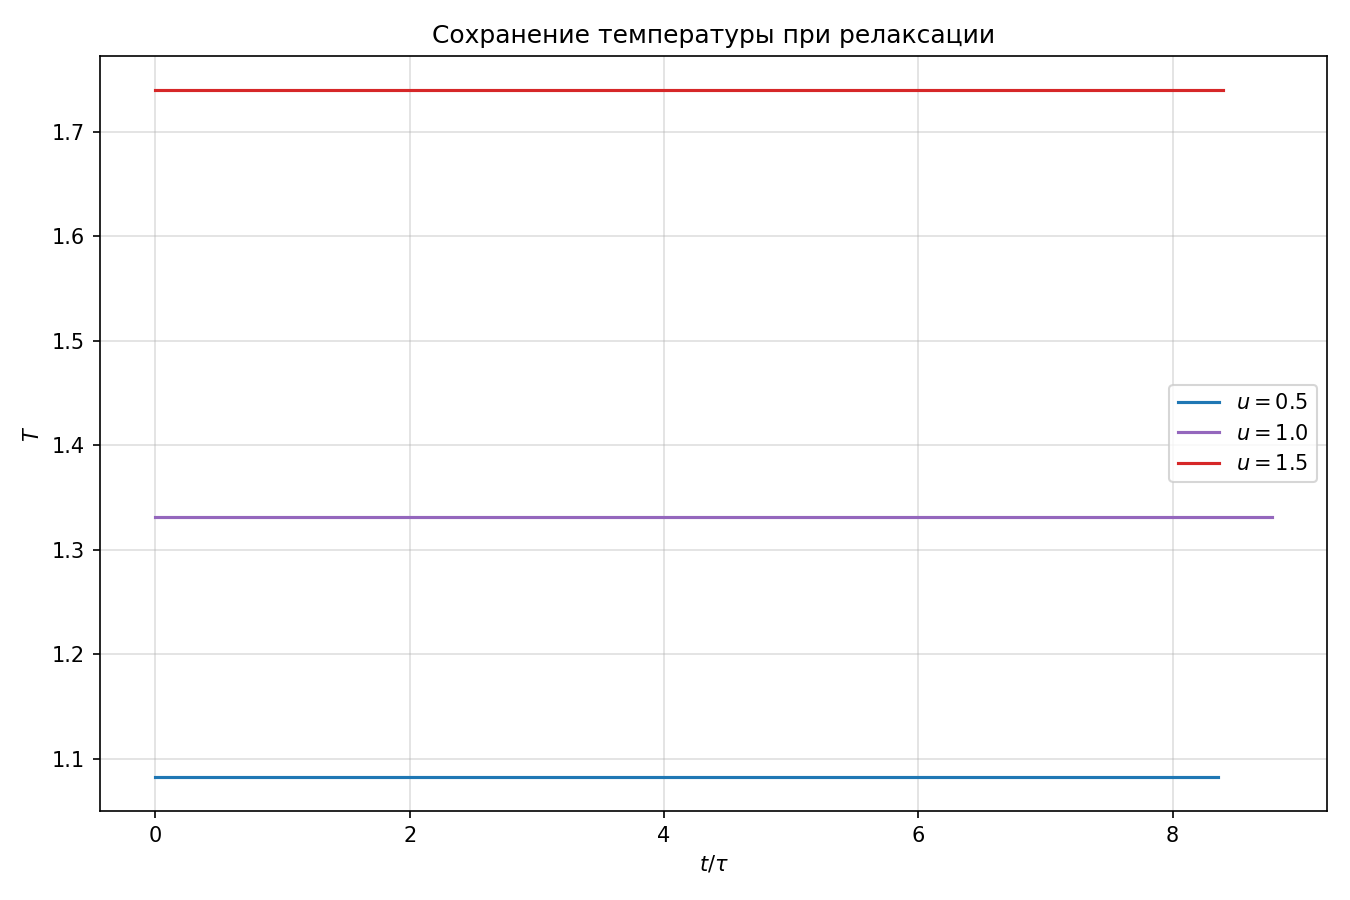
\includegraphics[width=\textwidth]{t0_T}
    \end{column}
  \end{columns}
\end{frame}

% 7. Верификация 1 — H-функция
\begin{frame}{Верификация 1. $H$-теорема}
  \centering
  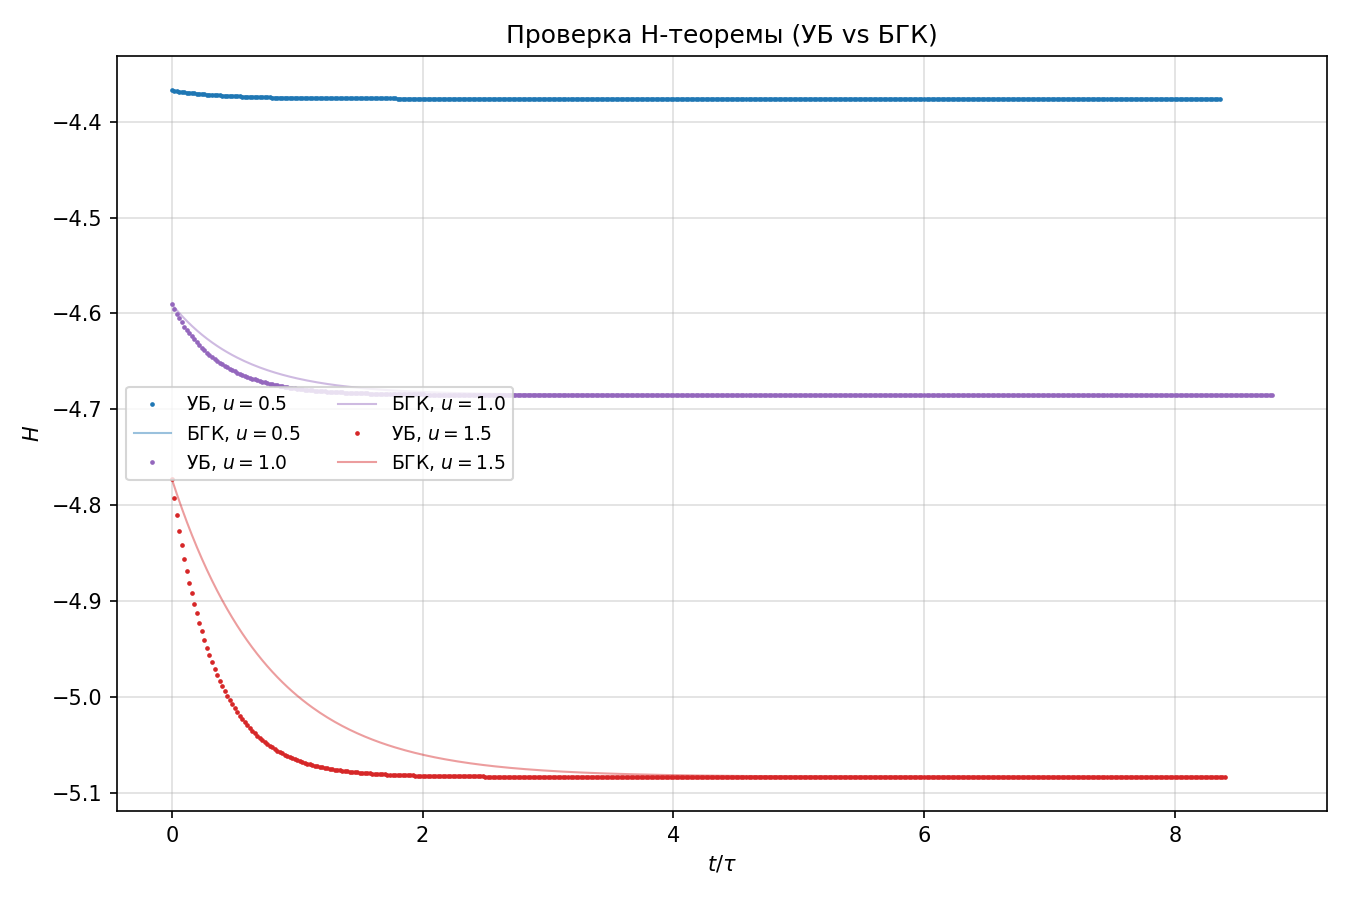
\includegraphics[width=0.62\textwidth]{t0_H}\\
  {\small $H$ монотонно невозрастает; скорость убывания растёт с параметром $u$.}
\end{frame}

% 8. Верификация 2 — смесь
\begin{frame}{Верификация 2. Бинарная смесь «холодный + горячий»}
  \begin{columns}
    \begin{column}{0.5\textwidth}
      \begin{itemize}\small
        \item $T_c=1$, $T_h=2$, $n_c=n_h=0{,}5$.
        \item Равновесие $T=\dfrac{\sum_i n_iT_i}{\sum_i n_i}=1{,}5$.
        \item Концентрации сохраняются; суммарная энтропия растёт.
      \end{itemize}
    \end{column}
    \begin{column}{0.5\textwidth}
      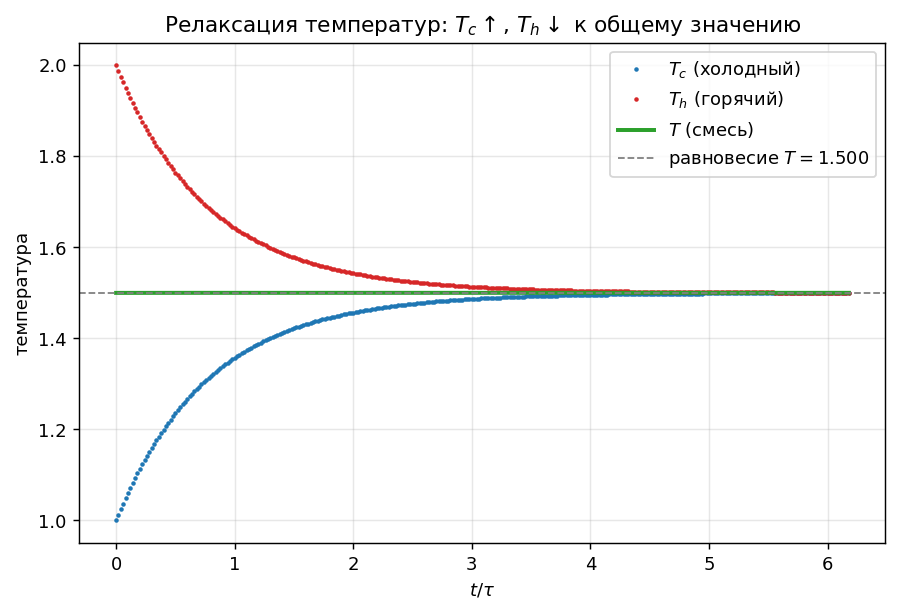
\includegraphics[width=\textwidth]{t1_T}
    \end{column}
  \end{columns}
\end{frame}

% 9. Верификация 2 — энтропия
\begin{frame}{Верификация 2. Рост энтропии смеси}
  \centering
  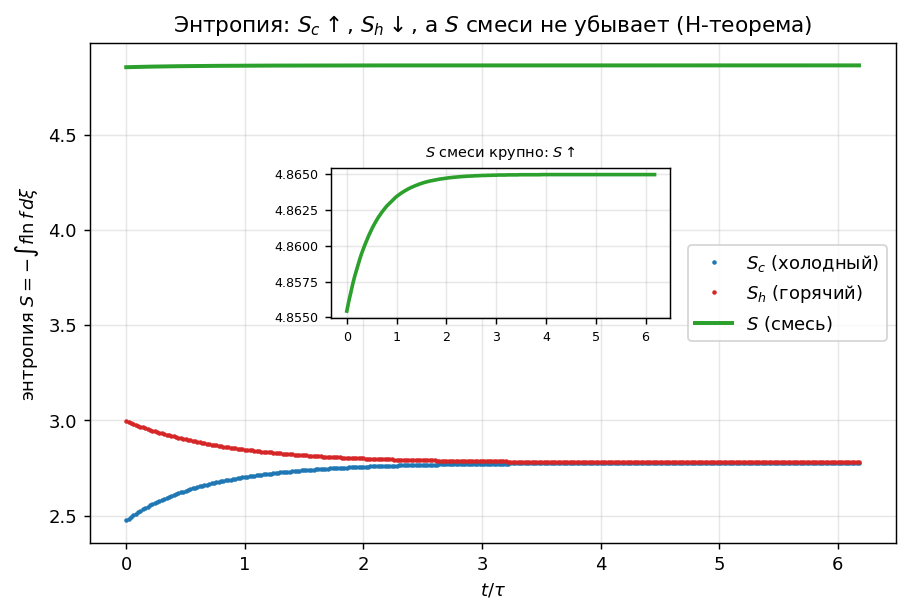
\includegraphics[width=0.6\textwidth]{t1_S}\\
  {\small Суммарная энтропия монотонно растёт ($H$-теорема); компоненты — противоположно.}
\end{frame}

% 10. Перенос — постановка
\begin{frame}{Задача переноса: ударная волна перед поршнем}
  \[ \frac{\partial f}{\partial t}+\xi_x\frac{\partial f}{\partial x}=I(f,f) \]
  \begin{itemize}
    \item Полупространство $x\le0$, поршень при $x=0$; набегающий поток $u_0=2c$ ($M=2$).
    \item Зеркальное отражение на стенке, набегающий максвелл слева.
    \item Теория Ренкина--Гюгонио: $M_s=3$, $n_1/n_0=3$, $T_1/T_0\approx3{,}66$.
  \end{itemize}
\end{frame}

% 11. Перенос — схема
\begin{frame}{Перенос: численная схема}
  \begin{itemize}
    \item \textbf{Расщепление Странга:} перенос$(\tfrac{\Delta t}{2})\to$ столкновения$(\Delta t)\to$
          перенос$(\tfrac{\Delta t}{2})$.
    \item \textbf{Перенос:} монотонная TVD-схема 2-го порядка, ограничитель MC,
          число Куранта $\le1$.
    \item \textbf{Столкновения:} тот же проекционный метод; в неоднородной задаче —
          4-кратная поперечная симметрия (ось $x$ выделена).
    \item Геометрия столкновений \textbf{предвычисляется} и применяется векторно ко всем ячейкам.
  \end{itemize}
\end{frame}

% 12. Перенос — результаты
\begin{frame}{Перенос: результаты (установившаяся УВ, $L=80$, $N_x=400$)}
  \centering
  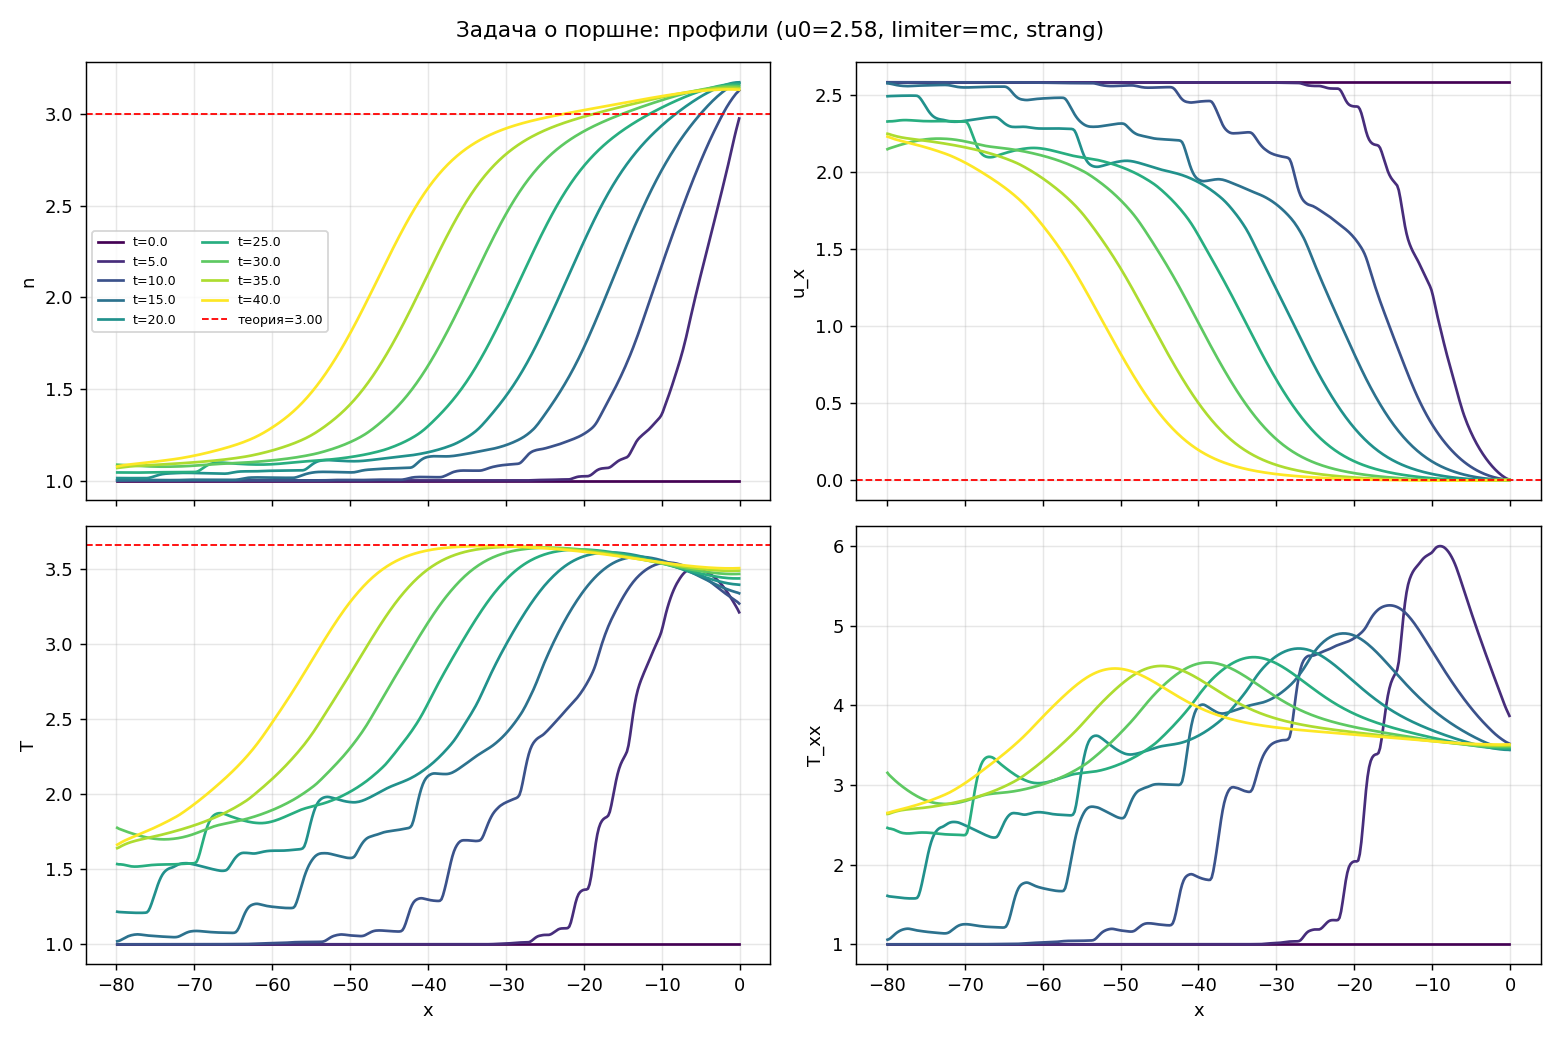
\includegraphics[width=0.82\textwidth]{t2_profiles}\\
  {\small Профили $n,\,u_x,\,T,\,T_{xx}$: сжатие $n\to3$, нагрев $T\to3{,}6$,
   кинетический «перескок» $T_{xx}$ на фронте.}
\end{frame}

% 13. Перенос — фронт, ФР и проверка Гюгонио
\begin{frame}{Перенос: фронт волны и проверка Гюгонио}
  \begin{columns}
    \begin{column}{0.52\textwidth}
      \centering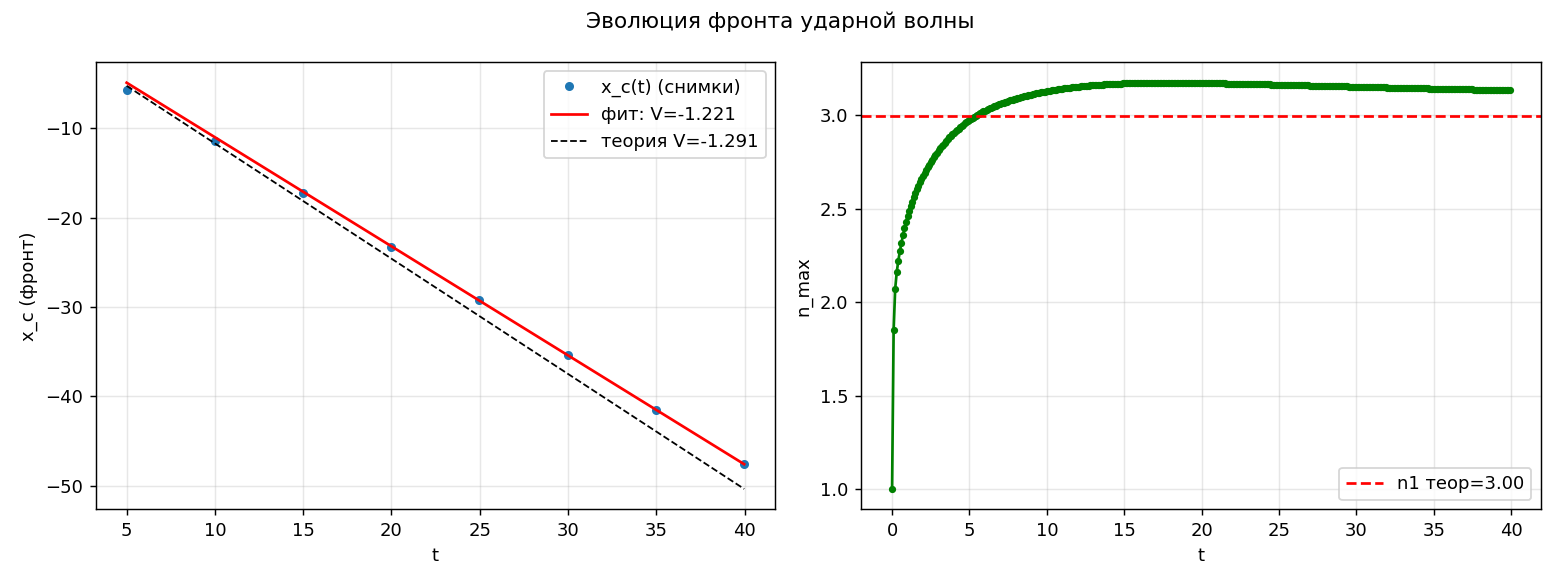
\includegraphics[width=\textwidth]{t2_front}\\
      {\small Фронт $x_c(t)$ линеен $\Rightarrow V$; \quad $n_{\max}\to3$.}
    \end{column}
    \begin{column}{0.48\textwidth}
      \centering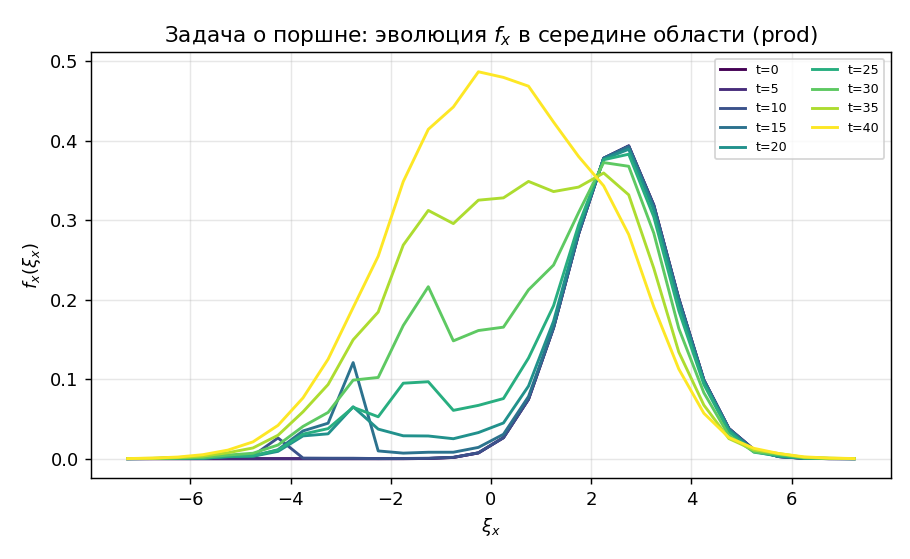
\includegraphics[width=\textwidth]{t2_fx}\\
      {\small $f_x$: холодный поток $\to$ горячий послескачковый газ.}
    \end{column}
  \end{columns}
  \vfill
  {\small \textbf{Согласие с теорией Ренкина--Гюгонио:} $n_1/n_0=2{,}95$ (теор.\ $3{,}0$),
   $T_1/T_0=3{,}62$ ($3{,}66$), $V=-1{,}22$ ($-1{,}29$); невязка $\sim2\,\%$.}
\end{frame}

% 14. Суперкомпьютер
\begin{frame}{Расчёты на суперкомпьютере}
  \begin{itemize}
    \item Кластер ЦКП НИЦ «Курчатовский институт» (раздел \texttt{hpc4-el7-3d}),
          система очередей \textbf{SLURM}, механизм \textbf{job-array}.
    \item Оптимизации под размер фазовой сетки: предвычисление геометрии, векторизация
          (\(\sim\)400$\times$ к скалярному коду), хранение «четвертью» (память $\times4\dots8$).
    \item \textbf{Структурная параллелизуемость:} интеграл столкновений независим по ячейкам
          и по узлам Коробова — естественное масштабирование.
    \item \textbf{Направление развития:} компилируемый солвер с MPI/GPU.
  \end{itemize}
\end{frame}

% 15. Заключение
\begin{frame}{Заключение}
  \begin{enumerate}
    \item Реализован консервативный проекционный метод; подтверждены строгие законы
          сохранения и $H$-теорема.
    \item Солвер верифицирован на задачах релаксации (квази-шок, смесь $T\to1{,}5$).
    \item Решена задача переноса: ударная волна перед поршнем; согласие с теорией
          Ренкина--Гюгонио ($n_1\approx3$, $T_1\approx3{,}6$, невязка $\sim2\,\%$).
    \item Расчёты проведены на суперкомпьютерном кластере; показана параллелизуемость метода.
  \end{enumerate}
  \vfill
  {\small \textbf{Апробация:} доклад и \textbf{призовое место} на 68-й Всероссийской научной
  конференции МФТИ (тезисы приняты к публикации).}
\end{frame}

% 16. Спасибо
\begin{frame}[plain]
  \centering
  \vfill
  {\Huge \textbf{Спасибо за внимание!}}\\[6mm]
  {\small Расчёты выполнены на оборудовании ЦКП НИЦ «Курчатовский институт».}
  \vfill
\end{frame}

\end{document}
